\documentclass{standalone}
\usepackage{tikz}

\begin{document}
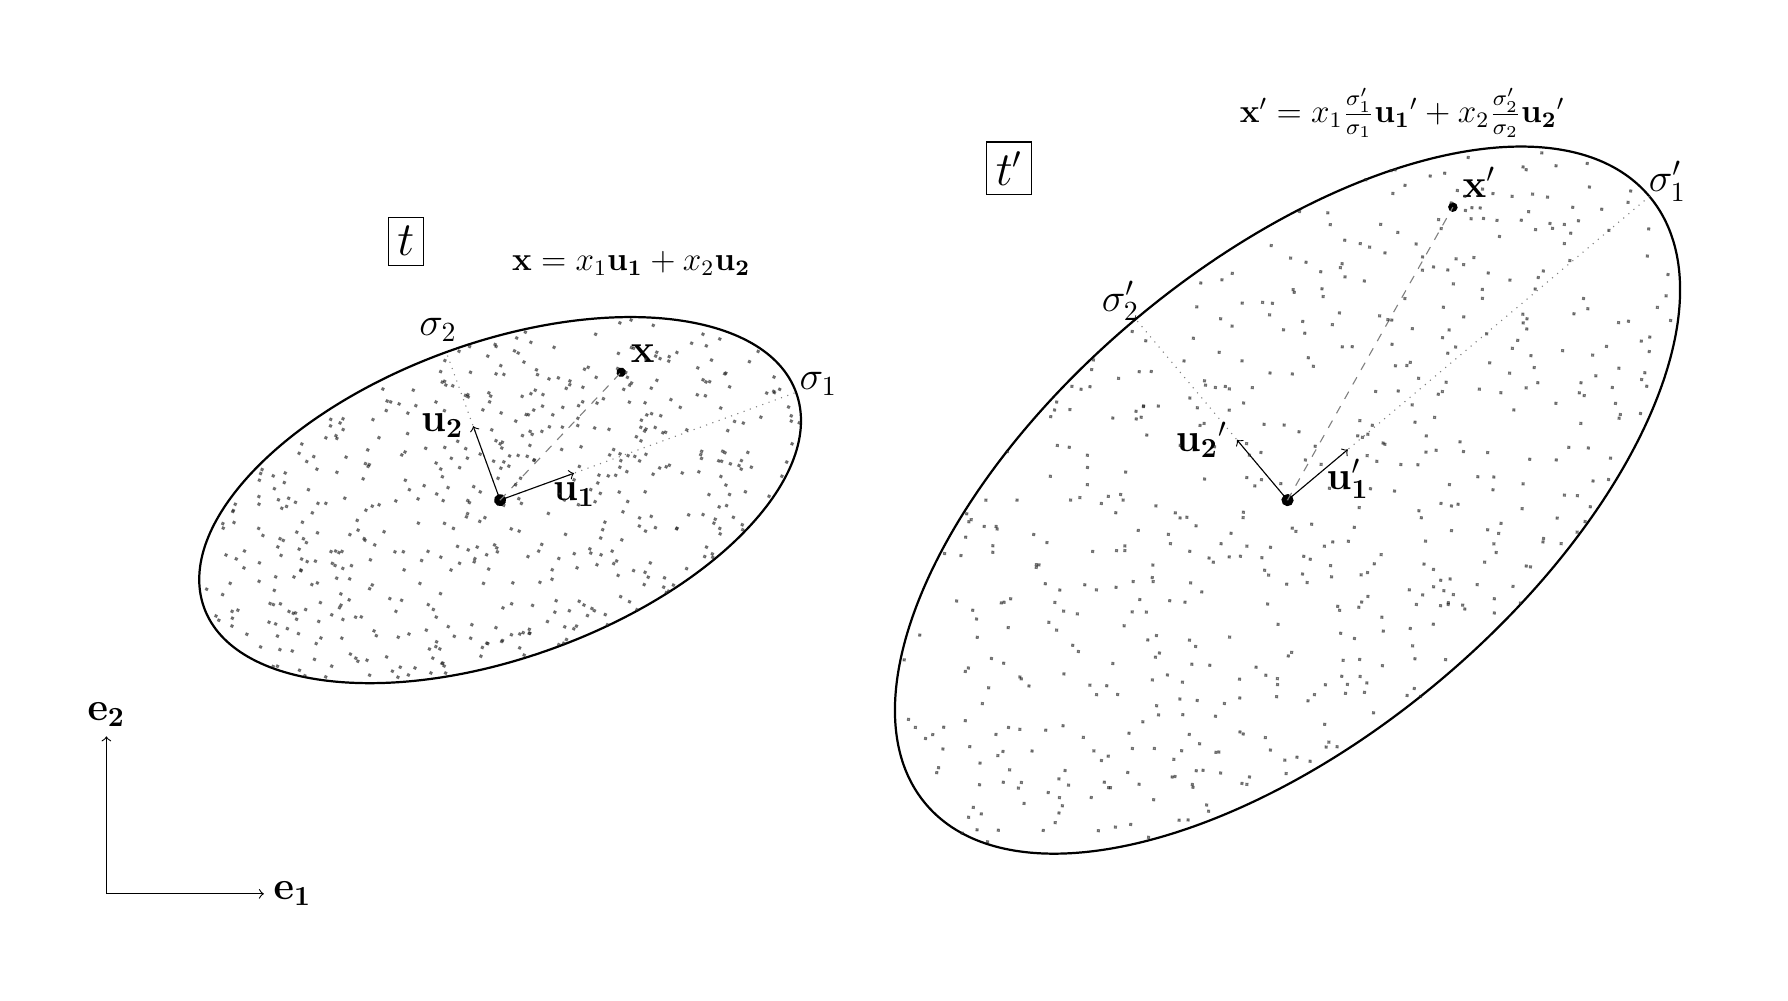
\begin{tikzpicture}[scale=1]

    % Set the canvas size
    \useasboundingbox (-6,-6) rectangle (16,6);

    % Define styles
    \tikzset{
        faint/.style={dotted, thin, gray},
        faint2/.style={dashed, thin, gray},
        vector/.style={-Latex, thick},
    }

    % First ellipse with 20 degrees rotation
    \begin{scope}[rotate=20]
        \draw[thick] (0,0) ellipse (4 and 2);
        \filldraw (0,0) circle (2pt);
        \draw[faint] (0,0) -- (4,0);
        \node[font=\fontsize{14}{14}\selectfont] at (4.3,0) {$\sigma_1$};
        \draw[faint] (0,0) -- (0,2);
        \node[font=\fontsize{14}{14}\selectfont] at (0,2.3) {$\sigma_2$};
        \draw[->] (0,0) -- (1,0) node[below,font=\fontsize{14}{14}\selectfont] {$\mathbf{u_1}$};
        \draw[->] (0,0) -- (0,1) node[left,font=\fontsize{14}{14}\selectfont] {$\mathbf{u_2}$};
        \coordinate (x) at (2,1);
        \filldraw (x) circle (1.5pt);
        \node[above right,font=\fontsize{14}{14}\selectfont] at (x) {$\mathbf{x}$};
        \draw[faint2] (0,0) -- (x);
        \node[above, font=\fontsize{12}{12}\selectfont] at (2.5, 2) {$\mathbf{x} = x_1 \mathbf{u_1} + x_2 \mathbf{u_2}$};
        \node[draw, font=\fontsize{16}{16}\selectfont] at (0, 3.5) {$t$};

        % Randomly distributed dots inside the first ellipse
        \foreach \i in {1,...,3000} {
            \pgfmathsetmacro{\x}{8*rand-4}  % Generate x within [-4, 4]
            \pgfmathsetmacro{\y}{4*rand-2}  % Generate y within [-2, 2]
            \pgfmathsetmacro{\test}{(\x/4)^2 + (\y/2)^2}
            \ifdim \test pt < 1pt
                \filldraw[fill=gray, opacity=0.5] (\x,\y) circle (0.5pt);
            \fi
        }
    \end{scope}

    % Second ellipse, translated and rotated
    \begin{scope}[xshift=10cm, rotate=40]
        \draw[thick] (0,0) ellipse (6 and 3);
        \filldraw (0,0) circle (2pt);
        \draw[faint] (0,0) -- (6,0);
        \node[font=\fontsize{14}{14}\selectfont] at (6.3,0) {$\sigma_1'$};
        \draw[faint] (0,0) -- (0,3);
        \node[font=\fontsize{14}{14}\selectfont] at (0,3.3) {$\sigma_2'$};
        \draw[->] (0,0) -- (1,0) node[below,font=\fontsize{14}{14}\selectfont] {$\mathbf{u_1'}$};
        \draw[->] (0,0) -- (0,1) node[left,font=\fontsize{14}{14}\selectfont] {$\mathbf{u_2}'$};
        \coordinate (x) at (4,1.5);
        \filldraw (x) circle (1.5pt);
        \node[above right,font=\fontsize{14}{14}\selectfont] at (x) {$\mathbf{x}'$};
        \draw[faint2] (0,0) -- (x);
        \node[above, font=\fontsize{12}{12}\selectfont] at (4, 2.5) {$\mathbf{x}' = x_1 \frac{\sigma_1'}{\sigma_1} \mathbf{u_1}' + x_2 \frac{\sigma_2'}{\sigma_2} \mathbf{u_2}'$};
        \node[draw, font=\fontsize{16}{16}\selectfont] at (0, 5.5) {$t'$};

        % Randomly distributed dots inside the second ellipse
        \foreach \i in {1,...,3000} {
            \pgfmathsetmacro{\x}{12*rand-6}  % Generate x within [-6, 6]
            \pgfmathsetmacro{\y}{6*rand-3}   % Generate y within [-3, 3]
            \pgfmathsetmacro{\test}{(\x/6)^2 + (\y/3)^2}
            \ifdim \test pt < 1pt
                \filldraw[fill=gray, opacity=0.5] (\x,\y) circle (0.5pt);
            \fi
        }
    \end{scope}

    % Axes e_1 and e_2
    \draw[->] (-5,-5) -- (-5,-3) node[above,font=\fontsize{14}{14}\selectfont] {$\mathbf{e_2}$};
    \draw[->] (-5,-5) -- (-3,-5) node[right,font=\fontsize{14}{14}\selectfont] {$\mathbf{e_1}$};

\end{tikzpicture}
\end{document}